\documentclass[a4paper, 11pt]{article}

%\usepackage[parfill]{parskip}
\usepackage{titlesec}
\newcommand{\sectionbreak}{\clearpage}
\usepackage{hyperref}
\usepackage{graphicx}
\usepackage{listings}
\usepackage[nounderscore]{syntax}
\usepackage{multirow}
\usepackage{chngpage}
\usepackage{array}
\usepackage{pbox}
\usepackage{amsmath}



\lstset{basicstyle=\footnotesize\ttfamily, columns=fullflexible, breaklines=true}

\graphicspath{ {images/} }


\makeatletter
\newcommand{\thickhline}{%
    \noalign {\ifnum 0=`}\fi \hrule height 1pt
    \futurelet \reserved@a \@xhline
}
\newcolumntype{"}{@{\hskip\tabcolsep\vrule width 1pt\hskip\tabcolsep}}
\makeatother

\newcommand\Tstrut{\rule{0pt}{3.3ex}}       % "top" strut
\newcommand\Bstrut{\rule[-1.3ex]{0pt}{0pt}} % "bottom" strut
\newcommand{\TBstrut}{\Tstrut\Bstrut} % top&bottom struts

\begin{document}

%------------------
% Title Page
%------------------
\begin{titlepage}
\newcommand{\HRule}{\rule{\linewidth}{0.5mm}}
\center

\textsc{\LARGE Birkbeck College}\\[1.5cm] % Name of your university/college

\textsc{\Large Msc Computer Science Project Report}

\HRule \\[0.4cm]
{ \LARGE \bfseries Learning and Video Games: Implementing an Evolutionary Agent}\\[0.4cm] % Title of your document
\HRule \\[1.5cm]


\begin{minipage}{0.4\textwidth}
\begin{flushleft} \large
\emph{Author:}\\
Monty \textsc{West} % Your name
\end{flushleft}
\end{minipage}
~
\begin{minipage}{0.4\textwidth}
\begin{flushright} \large
\emph{Supervisor:} \\
Dr. George \textsc{Magoulas} % Supervisor's Name
\end{flushright}
\end{minipage}\\[4cm]

\emph{MSc Computer Science project report, Department of
Computer Science and Information Systems, Birkbeck College,
University of London 2015}

\vspace{5mm}

\emph{This report is substantially the result of my own work,
expressed in my own words, except where explicitly indicated in
the text. I give my permission for it to be submitted to the
JISC Plagiarism Detection Service.}

\vspace{5mm}

\emph{The report may be freely copied and distributed provided the
source is explicitly acknowledged.}

\end{titlepage}

%------------------
% Abstract
%------------------

\begin{abstract}
Artificial intelligence in video games has long shunned the use of machine learning in favour of a handcrafted approach. However, the recent rise in the use of video games as a benchmark for academic AI research has demonstrated interesting and successful learning approaches. This project follows this research and explores the viability of a game-playing learning AI. Considering previous approaches, an evolutionary agent was created for a platform game based on Super Mario Bros.

The project builds on top of software developed for the Mario AI Competition, which provides the game-engine and agent interface, as well as several other pertinent features. The basic agent was constructed first and a learning framework was built to improve it, utilising a genetic algorithm. The project followed an agile methodology, revisiting design by analysing learning capability.

The aim was to produce an agent that shows meaningful improvement during learning and demonstrated unforeseen behaviours. 

!ADD EVAL HERE!

\end{abstract}

\vspace{10mm}

\iffalse
\begin{center}

\includegraphics[scale=0.3]{mario}  %What are you doing, remove this.
\end{center}
\fi

\clearpage

%------------------
% Contents
%------------------

\tableofcontents
\clearpage

%-------------------------------------------------------------------------
% Introduction (Brief Description of Topic + Fits in Field)
%-------------------------------------------------------------------------


\section{Introduction}

Artificial intelligence (AI) is a core tenant of video games, traditionally utilised as adversaries or opponents to human players. Likewise, game playing has long been a staple of AI research. However, academic research has traditionally focused mostly on board and card games and advances in game AI and academic AI have largely remained distinct.

The first video game opponents were simple discrete algorithms, such as the computer paddle in \emph{Pong}. In the late 1970s video game AIs became more advanced, utilising search algorithms and reacting to user input. In \emph{Pacman}, the ghost displayed distinct personalities and worked together against the human player \cite{pacmanghosts}. In the mid 1990s, approaches became more `agent' based. Finite State Machines (FSMs) emerged as a dominant game AI technique, as seen in games like \emph{Half-Life} \cite{halflife}. Later, in the 2000s, Behaviour Trees gained preeminence, as seen in games such as \emph{F.E.A.R.} \cite{fear} and \emph{Halo 2} \cite{halo}. These later advances borrowed little from contemporary development in academic AI and remained localised to the gaming industry.

However, with increases in processing power and the complexity of games over the last ten years many academic techniques have been harnessed by developers. For example, Monte Carlo Tree Search techniques developed for use in Go AI research has been used in \emph{Total War: Rome II} \cite{rome}. In 2008's \emph{Left 4 Dead}, Player Modelling was used to alter play experience for different users \cite[p.~10]{playermod}. Furthermore, AI and related techniques are no longer only being used as adversaries. There has been a rise in intelligent Procedural Content Generation in games in recent years, in both a game-world sense (for example \emph{MineCraft} and \emph{Terraria}) and also a story sense (for example \emph{Skyrim's} Radiant Quest System) \cite{skyrim}.

Moreover, games have recently enjoyed more consideration in academic research. Commercial games such as \emph{Ms. Pac Man}, \emph{Starcraft}, \emph{Unreal Tournament} and \emph{Super Mario Bros.} and open-source games like \emph{TORCS} \cite{torcs} and \emph{Cellz} \cite{cellz} have been at the centre of recent competitions and papers \cite{panorama} \cite{marioaicomp}. 

Learning has long been a staple of academic research into AI and dynamic programming, especially in robotics and board games. However, it has also had success in more niche problems, such as helicopter control \cite{rlheli} and human-computer dialogue \cite{rlhci}. Similarly the agent model is a popular approach to AI problems. It is seen in commercial applications, as mentioned above, as well as academic applications, such as board game AI. Furthermore, the agent model's autonomous nature makes it particularly suited to utilising biologically inspired learning.


%-----------------------------------------------------------------------
% Definitions
%-----------------------------------------------------------------------
\subsection{Concept Definitions}

At this point it is useful to introduce some high level descriptions/definitions of some key concepts.

\subsubsection{Intelligent Agents (IAs)}

\begin{figure}[t]
	\centering
	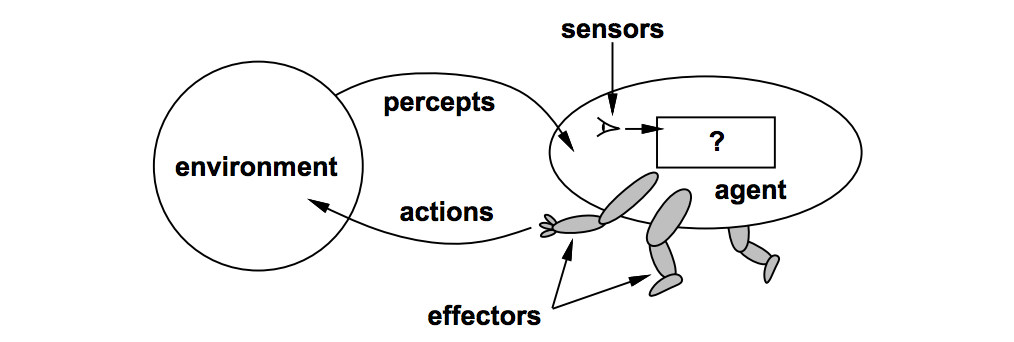
\includegraphics[scale=0.6]{intelligentagent.png}
	\caption{Illustration of an intelligent agent, taking from \cite[p.~32]{modernai1}}
	\label{fig:ia}
\end{figure}

An intelligent agent is an entity that uses \textbf{sensors} to perceive its \textbf{environment} and acts based on that perception through \textbf{actuators} or \textbf{effectors}. In software, this is often realised as an autonomous program or module that takes its perception of the \textbf{environment} as input an returns \textbf{actions} as output. Figure \ref{fig:ia} shows the basic structure of an intelligent agent. \cite[p.~34]{modernai3}


\subsubsection{Rule-based systems}

A rule-based system decides \textbf{actions} from \textbf{inputs} as prescribed by a \textbf{ruleset} or \textbf{rule base}. A \textbf{semantic reasoner} is used to manage to the relationship between input and the ruleset. This follows a \textbf{match-resolve-act} cycle, which first finds all rules matching an input, chooses one based on a conflict strategy and then uses the rule to act on the input, usually in the form of an output. \cite[pp.~28-29]{rbsys}

\subsubsection{Biologically Inspired Learning} 

Several computational learning approaches have derived their inspiration from learning in animals and humans. Two such approaches are relevant to this project: Reinforcement learning, strategy modelled on simplistic interpretation of how animal learn behaviour from their environment \cite[s.~1.2]{suttonrl}; and evolutionary computation, algorithms that apply Darwinian principles of evolution \cite{ev-comp}.


\subsubsection{Reinforcement Learning}

A reinforcement learning agent focuses on a learning problem, with its goal to maximise \textbf{reward}. Given a current \textbf{state} the agent chooses an \textbf{action} available to it, which is determined by a \textbf{policy}. This action maps the current \textbf{state} to a new \textbf{state}. This \textbf{transition} is then evaluated for its \textbf{reward} . This \textbf{reward} often affects the \textbf{policy} of future iterations, but \textbf{policies} may be stochastic to some level. \cite[s.~1.3]{suttonrl}

\subsubsection{Evolutionary Computation}

The evolutionary computation encompasses many learning algorithms, two of which are described in detail below. The process looks to optimise a data representation of the problem through random variation and selection in a \textbf{population}. It commonly employs techniques similar to survival, breeding and mutation found in biological evolutionary theory.  \cite{ev-comp}

\subsubsection{Online/Offline Learning}
\begin{description}
	\item[Offline] An offline (or batch) learner trains on an entire dataset before applying changes. 
	\item[Online] A online learner reacts/learns from data immediately after each datapoint.
\end{description} 
	
\subsubsection{Genetic Algorithms (GAs)}

Genetic Algorithms are an subset of evolutionary computation. They model the solution as a \textbf{population} of \textbf{individuals}. Each \textbf{individual} has a set of \textbf{genes} (a  \textbf{genome}), which can be thought of as simple pieces of analogous information (most often in the form of bit strings). Each \textbf{individual} is assessed by some \textbf{fitness function}. This assessment can be used to cull the \textbf{population}, akin to survival of the fittest, or to increase the individual's chance of influencing the next \textbf{population}. The new \textbf{population} is created by \textbf{breeding}, using a combination of the following: \textbf{crossover} of the \textbf{genome} from two (or more) \textbf{individuals} (akin to sexual reproduction), \textbf{mutation} of the \textbf{genes} of one \textbf{individual} (akin to asexual reproduction) and \textbf{re-ordering} of the \textbf{genes} of one \textbf{individual}. Each new \textbf{population} is called a \textbf{generation}. \cite[p.~7]{mitchellga}

\subsubsection{Evolution Strategies (ESes)}

Evolution Strategies differ from standard Genetic Algorithms by using \textbf{truncation selection} before breeding. The top $\mu$ individuals of the population are chosen (usually by fitness) and bred to create $\lambda$ children. ES notation has the following form:  $\pmb{(\mu / \rho \  \overset{+}{,} \  \lambda)}$. $\rho$ denotes the number of individuals from $\mu$ used in the creation of a single $\lambda$, (i.e. number of parents of each child) this report will only consider the case $\rho = 1$. The $+$ and $,$ are explained below:  \cite[p.~6-10]{es-book} \cite[s.~4.1.2]{ecj-manual}
\begin{description}
	\item[$\pmb{(\mu \  , \   \lambda)}$]  Denotes an ES that has a population size of lambda. The top $\mu$ individuals are taken from the $\lambda$ in generation $g-1$, which then produce $\lambda$ children for generation $g$. This is done by creating $\lambda / \mu$ clones of each $\mu$ and then mutating them individually. 
	\item[$\pmb{(\mu  + \lambda)}$] Differs from the $\pmb{(\mu \  , \   \lambda)}$ variant by adding the $\mu$ individuals chosen from generation $g-1$ to the new generation $g$ after the mutation phase. Hence the population size is $\lambda + \mu$.
\end{description}


%-----------------------------------------------------------------------
% Motivation
%-----------------------------------------------------------------------
\subsection{Motivation}

Exploring the use of learning techniques for use in video games is a challenging and eminent area of research, with interest from both the video game and computation intelligence communities.

\subsubsection*{Desirability}

Ventures in utilising learning in commercial video games have been limited and largely ineffectual. However, there are many reasons why good execution of these techniques is desirable. Firstly, modern games have large and diverse player bases, having a game that can respond and personalise to a specific player can help cater to all. Secondly, learning algorithms produce agents that can respond well in new situations (over say FSMs or discrete logic), hence making new content easy to produce or generate. Lastly, humans must learn and react to environments and scenarios during games. Having non-playable characters do the same may produce a more believable, immersive and relatable AI, which is one of the key criticisms with current games. \cite[p.~7, p.~13]{panorama}

\subsubsection*{Issues}

The main issue with constructing effectual learning (or learnt) agent AI in game is risk versus reward. Game development works on strict cycles and there are limited resources to invest into AI research, especially if the outcome is uncertain. Furthermore, one player playing one game produces a very small data set, making learning from the player challenging. Moreover, AI that is believably human is a field still in its infancy. \cite{evolutioningamedesign}

\subsubsection*{Games as a Benchmark}

Despite the lack of commercial success, video games can act as great benchmark for learning agents. They are designed to challenge humans, and therefore will challenge learning methods, especially those inspired by biological processes. Games naturally have some level of learning curve associated with playing them (as a human). Also, games require quick reactions to stimulus, something not true of traditional AI challenges such as board games. Most games have some notion of scoring suitable for a fitness function. Lastly, they are generally accessible to students, academics and the general public alike. \cite[p.~9]{panorama} \cite[p.~1]{marioaicomp} \cite[p.~2]{2012the}

\vspace{\baselineskip}

As such, games have now been utilised in several academic AI competitions. These competitions are the forefront of research and development into learning techniques in video games, and will be explored in more detail in section \ref{subsec:gameaicomps}.

This project is motivated by the variety of previous approaches taken in these competitions and the unexpected results they produced. 


%-----------------------------------------------------------------------
% Aims and Objectives
%-----------------------------------------------------------------------
\subsection{Aim and Objectives}

The aim of the project is to explore the use of behavioural learning techniques in creating a game-playing agent-based AI. This will be achieved by producing an intelligent agent, developed by a evolutionary algorithm, that plays a 2D side-scrolling platform game.

\subsubsection*{Objectives}

\begin{enumerate}

	\item \label{obj:design}
	\textbf{Design} \\
	Influenced by previous approaches, design an agent and learning procedure that can demonstrate meaningful improvement during learning.
	
	\item \label{obj:impl}
	\textbf{Implementation} \\
	Implement agent and learning designs in a modular, customisable and test-driven manner, utilising external libraries and features of the game software.
	
	\item \label{obj:test}
	\textbf{Testing} \\
	Provide significant test coverage to the functionality of the implementation.
	
	\item \label{obj:learn}
	\textbf{Learning} \\
	Grant the agent a large and diverse testbed from which to learn as well as ample time and resources to do so.
	
	\item \label{obj:eval}
	\textbf{Evaluation} \\
	Evaluate both the competence and learning capability of the agent and compare to alternative approaches.

\end{enumerate}

%-----------------------------------------------------------------------
% Methodology
%-----------------------------------------------------------------------
\subsection{Methodology}

The two central components to this project, the agent and the learning process, will be designed, implemented and tested as two separate modules. This presents a clean separation of concerns. The agent module will be completed first, followed by the learning module. A third module will also be created, which will allow the agent to play generated levels and receive a score.

The Mario benchmark software is open-source\footnote{Available at http://www.marioai.org/gameplay-track/getting-started} and will form the initial codebase for this project. It is written in Java and contains the game-engine and useful features such as level generation and level playing classes.

I intend to use Scala as the main language of this project as I believe that it's functional and concurrent features will suit the problem. Scala and Java are widely compatible (as they both compile JVM bytecode) so this should not require a significant amount of work. However, the codebase will be assessed for the suitability of this approach, and Java 8 will be used if Scala proves to be counterproductive.

Furthermore the software will be assessed for the inclusion of build tools, such as \emph{sbt} and \emph{Maven}; testing frameworks, such as \emph{ScalaMock} and \emph{Mockito} and logging, such as \emph{log4j} and Scala's inbuilt logging package.

\subsubsection*{Objective \ref{obj:design}: Design}
\label{meth:design}

The design of both the agent and learning module will follow the approach of the REALM agent, discussed in \ref{ssec:realm}.

The agent module will be a rule-based system that maps environment based conditions to explicit key presses. This project will look to differ from the REALM agent in regards to specific environment perceptions. The available sensory information will be assessed and distilled into a collection of simple observations.

The learning module will utilise an offline genetic algorithm with a similar configuration seen in \ref{ssec:realm}. Agents will be individuals, with rulesets as genomes. Fitness of an individual will be determined by playing generated levels. However, different approaches to mutation, crossover and reordering will be explored, as well as careful consideration of calculating fitness from level playing statistics.

\subsubsection*{Objective \ref{obj:impl}: Implementation}
\label{meth:impl}

The agent module will implement the \emph{Agent} interface including in the benchmark, which will allow for the agent to used in other areas of the benchmark software, such as the game-playing and evaluation classes. Each agent will be defined by it's ruleset, the contents of which will determine its behaviour. The agent will implement a semantic reasoner for the ruleset, returning a action as prescribed by the chosen rule.

The agent will gather it's sensory information from the game's \emph{Environment} class, which reports visible properties of the level scene. As discussed in \ref{meth:design}, this will be simplified to a list of observations and compared against the agent's ruleset.

\vspace{\baselineskip}

The learning module will utilise an external library alongside the level playing module. Many evolutionary computation libraries exist for Java (and therefore Scala), \emph{ECJ} \cite{ecj} and \emph{JGAP} \cite{jgap} will both be considered for use in this project.

The implementation will manage the integration of this library with both the agent and level playing modules. The algorithm will evolve a simple data structure representation of rulesets, inject them into agents and assess those agents by having them play several carefully parametrised levels. The statistics returned from these levels will form the base variables of the fitness function, with multipliers being configurable. To aid in improving the learning process, these parameters will be held 
externally and fitness values will be logged.

\subsubsection*{Objective \ref{obj:test}: Testing}
\label{meth:test}

Test coverage the agent module will handled by black-box testing. Unit tests will be written to test the semantic reasoner and the environment observation methods.

Due to the stochastic nature of genetic algorithms, testing of the learning module will be limited. However, the breeding can be tested by verifying that children stay within parameters. Some evolutionary libraries, such as JGAP, provide several unit tests. If available these will become the primary source of test coverage for the module.

\subsubsection*{Objective \ref{obj:learn}: Learning}
\label{meth:learn}

Optimising the learning parameters, including the parameters of the breeding phase, fitness function and level playing, will be an important stage of the project. Assessment of the parameters used in previous agent such as REALM (discussed in \ref{ssec:realm}) D. Perez et al. \cite{gramev} and Agent Smith \cite{agentsmith} will inform the initial values. From there learning module logs will be analysed for improvements. For example, if there is a lot of variation in fitness then perhaps mutation should be restricted, or if the average fitness does not eventually level out then the further generations should be created.

The design of the agent can also influence the effectiveness of the learning algorithm. The size of the search space is determined by the conditions and actions of the rulesets, the reduction of which could improve evolutionary capability. Hence, the learning phase of the project may inform a redesign of the agent, which is one of the main reasons this project will take an agile approach.

The learning itself is likely to be a time consuming, computationally heavy procedure. To assist in providing ample resources to this process the project will have access to two 8 core servers, as well as a laptop with an Intel i7 processor.

\subsubsection*{Objective \ref{obj:eval}: Evaluation}
\label{meth:eval}

On the conclusion of the learning process the best/final agent will be extracted and evaluated. This will be done by using the level playing module. The agent will go through an extensive set of levels, based on the approach taken by the 2010 Mario AI Competition.

The primary comparison will be with a handcrafted ruleset, which will assess the significance of the agent evolution. Other comparisons can be drawn against agents that are included as examples in the benchmark, such as the \emph{ForwardJumpingAgent} that was used for similar comparisons in the 2009 competition, as well as other entrants into the competition.

The second part of this objective is to evaluate the learning procedure. Figures such as average and maximum generation fitness can provide an insight into the effectiveness of the genetic algorithm. Furthermore, a baseline for these values can be provided by having the handcrafted agent play the levels alongside the evolving agent. The final evaluation report will provide an analysis of these figures.

%-----------------------------------------------------------------------
% Report Structure
%-----------------------------------------------------------------------
\subsection{Report Structure}

This report will cover previous approaches to the project's aim; the design, implementation of the agent and learning process; and evaluate both the results and the project as a whole.

Section 2 details existing work, specifically relevant entrants to Game AI competitions. It will consider their approaches to both learning and agent design for both effectiveness and significance to learning in video games. It will look in particular at the Mario AI Competition and the winner entrant in 2010, the REALM agent.

Section 3 will cover the projects specification, discussing functional and non-functional requirements. It will also include a description of the major dependencies that influenced project design.

Section 4 will explain the design, implementation and testing of the rule-based agent. It will demonstrate how the agent was built to allow it be evolved by a genetic algorithm, as well as how it perceives its environment and choosing an action. Reasons for the choice of project language and build tools is also included here. 

Section 5 will detail the development of the level playing module.This contains an account of the modifications that had to be made to the game engine software. It covers the extension to the game engine and how it as designed and implemented with a view to parametrisation and level variety.

Section 6 explains the choice of genetic algorithm and the basic parameters used. It also describes extensions made to the learning library to allow it to effectively evolve the agent in an easily customisable and observable fashion. Lastly, it details how specific mutataion and fitness parameters were chosen in response to initial learning runs in order to improve the process.

Section 7 evaluates the agent framework for it's capability by considering 3 hand crafting agent rulesets. It then compares these agents to the final learnt agent, assessing it for attainment, as well as interesting and unexpected behaviour. It also studies the effectiveness of the learning algorithm by examining metrics such as fitness increase over generations. Finally, it concludes with an analysis of the project as a whole, with a discussion on extensions and improvements to the learning and agent modules and the overall methodology.

\clearpage

%___________________________________________
%*************************************************************
% Existing Work
%___________________________________________
%^^^^^^^^^^^^^^^^^^^^^^^^^^^^^^^^^^^^^^^^^^^^^^^^^^^

\section{Existing Work}

%-----------------------------------------------------------------------
% Learning in Games (Current Work in Field)
%-----------------------------------------------------------------------

\subsection{Learning Agents and Game AI Competitions}
\label{subsec:gameaicomps}

Over the last few years several game based AI competitions have been run, over a variety of genres. These competitions challenge entrants to implement an agent that plays a game and is rated according to the competitions specification. They have attracted both academic \cite[p.~2]{2012the} and media interest \cite[p.~2]{marioaicomp}. The competition tend to encourage the use of learning techniques. Hence, several interesting papers concerning the application of biologically inspired learning agents in video games have recently been published. Approaches tend to vary widely, modelling and tackling the problem very differently and specialising techniques in previously unseen ways. \cite[p.~11]{2012the}

Some brief details of the competitions which are of relevance to this project are compiled in to Table \ref{tab:gameaicomp}. The Mario AI Competition is also explored in more detail below.

\begin{table}
  \begin{adjustwidth}{-4cm}{-4cm}
  \begin{center} \small
    \begin{tabular}{ | >{\raggedright}p{2cm} | >{\raggedright}p{2cm} | p{7.5cm} |}
    \hline
    \textbf{Genre} & \textbf{Game} & \textbf{Description} \TBstrut \\ \thickhline
    Racing & TORCS (Open-source) \cite{torcs} &  
    \textbf{The Simulated Car Racing Competition}\newline Competitors enter agent drivers, that undergo races against other entrants which include qualifying and multi-car racing. The competition encourages the use of learning techniques. \cite{scrc}
      \\ \hline
    First Person Shooter (FPS) & Unreal Tournament 2004 &
    \textbf{The 2K BotPrize}\newline Competitors enter `bots' that play a multi-player game against a mix of other bots and humans. Entrants are judged on Turing test basis, where a panel of judges attempt to identify the human players. \cite{2kbot}
       \\ \hline
    Real Time Strategy (RTS) & Starcraft &
    \textbf{The Starcraft AI Competition}\newline Agents play against each other in a 1 on 1 knockout style tournament. Implementing an agent involves solving both micro objectives, such as path-planning, and macro objectives, such as base progression. \cite{starcomp}
       \\ \hline
    Platformer & Infinite Mario Bros (Open-source) &
    \textbf{The Mario AI Competition}\newline Competitors submit agents that attempt to play (as a human would) or create levels. The competition is split into `tracks', including Gameplay, Learning, Turing and Level Generation. In Gameplay, each agent must play unseen levels, earning a score, which is compared to other entrants. \cite{2012the} 
       \\ \hline
    
    \end{tabular}
  \end{center}
  \end{adjustwidth}
  \caption{This table summarises some recent game AI competitions \cite{2014how}}
  \label{tab:gameaicomp}
\end{table}

\subsubsection{The Mario AI Competition}
\label{subsec:marioaibench}

The Mario AI Competition, organised by Sergey Karakovskiy and Julian Togelius, ran between 2009-2012 and used an adapted version of the open-source game Infinite Mario Bros. From 2010 onwards the competition was split into four distinct `tracks'. We shall focus on the unseen Gameplay track, where agents play several unseen levels as Mario with the aim to finish the level (and score highly). \cite{marioaicomp} \cite{2012the}

\subsubsection*{\hspace{6pt}Infinite Mario Bros.}

Infinite Mario Bros (IMB) \cite{imb} is an open-source clone of Super Mario Bros.~3, created by Markus Persson. The core gameplay is described as a \emph{Platformer}. The game is viewed side-on with a 2D perspective. Players control Mario and travel left to right in an attempt to reach the end of the level (and maximise score). The screen shows a short section of the level, with Mario centred. Mario must navigating terrain and avoid enemies and pits. To do this Mario can move left and right, jump, duck and speed up. Mario also exists in 3 different states, \emph{small}, \emph{big} and \emph{fire} (the latter of which enables Mario to shoot fireballs), accessed by finding powerups. Touching an enemy (in most cases) reverts Mario to a previous state. Mario dies if he touches an enemy in the \emph{small} state or falls into a pit, at which point the level ends. Score is affected by how many coins Mario has collected, how many enemies he has killed (by jumping on them or by using fireballs or shells) and how quickly he has completed the level. \cite[p.~3]{2012the}

\subsubsection*{\hspace{6pt}Suitability to Learning}

The competitions adaptation of IMB (known henceforth as the `benchmark') incorporates a tuneable level generator and allows for the game to be sped-up by removing the reliance on the GUI and system clock. This makes it a great testbed for reinforcement learning. The ability to learn from large sets of diverse data makes learning a much more effective technique. \cite[p.~3]{2012the}

Besides that, the Mario benchmark presents an interesting challenge for learning algorithms. Despite only a limited view of the ``world" at any one time the state and observable space is still of quite high-dimension. Though not to the same extent, so too is the action space. Any combination of five key presses per timestep gives a action space of $2^5$ \cite[p.~3]{2012the}. Hence part of the problem when implementing a learning algorithm for the Mario benchmark is reducing these search spaces. This has the topic of papers by Handa and Ross and Bagnell \cite{rossbagnell} separately addressed this issue in their papers \cite{handa} and \cite{rossbagnell} respectively.

Lastly, there is a considerable learning curve associated with Mario. The simplest levels could easily be solved by agents hard coded to jump when they reach an obstruction, whereas difficult levels require complex and varied behaviour. For example, traversing a series of pits may require a well placed series of jumps, or passing a group of enemies may require careful timing. Furthermore, considerations such as score, or the need to backtrack from a dead-end greatly increase the complexity of the problem. \cite[p.~3, p.~12]{2012the}


%-----------------------------------------------------------------------
% Previous Agents
%-----------------------------------------------------------------------

\subsection{Previous Learning Agent Approaches}
\label{ssec:prevagents}

Agent-based AI approaches in commercial games tend to focus on finite state machines, behaviour trees and rulesets, with no learning component. Learning agents are more prevalent in AI competitions and academia, where it is not only encouraged, but viewed as an interesting research topic \cite[p.~1]{marioaicomp}. Examples from both standpoints are compiled in Table \ref{tab:agents}.

\subsubsection{Evolutionary Algorithms}

Evolutionary algorithms are a common choice of learning methods used in game-playing agents. D. Perez et al. note in their paper \cite[p.~1]{gramev} that they are particular suitable for game environments: 
\begin{quote}\itshape
`Their stochastic nature, along with tunable high- or low-level representations, contribute to the discovery of non-obvious solutions, while their population-based nature can contribute to adaptability, particularly in dynamic environments.'
\end{quote}
The evolutionary approach has been used across several genres of video games. For example, \emph{neuroevolution}, a technique that evolves neural networks, was used in both a racing game agent (by L. Cardamone \cite[p.~137]{scrc}) and a FPS agent (by the UT$\wedge$2 team \cite{2kbot}). Perhaps the most popular approach was to use genetic algorithms (GAs) to evolve a more traditional game AI agent. R. Small used a GA to evolve a ruleset for a FPS agent \cite{agentsmith}, T. Sandberg evolved parameters of a potential field in his Starcraft agent \cite{emapf} , \emph{City Conquest's} in-game AI used an agent-based GA-evolved build plan \cite{evolutioningamedesign} and D. Perez et al. used a grammatical evolution (a GA variant) to produce behaviour trees for a Mario AI Competition entry \cite{gramev}.

\subsubsection{Multi-tiered Approaches}

Several of the most successful learning agents take a multi-tiered approach. By splitting high-level behaviour from low-level actions agents can demonstrate more a complex, and even human-like, performance. For example, COBOSTAR, an entrant in the 2009 Simulated Car Racing Competition, used offline learning to determine high-level parameters such as desired speed and angle alongside a low-level crash avoidance module \cite[p.~136]{scrc}. UT$\wedge$2 used learning to give their FPS bot broad human behaviours and a separate constraint system to limit aiming ability \cite{2kbot}.  Overmind, the winner of the 2010 Starcraft Competition, planned resource use and technology progression at a macro level, but used A* search micro-controllers to coordinate units \cite{overmind}. 

\vspace{\baselineskip} \noindent
One learning agent that successfully utilised both an evolutionary algorithm and a multi-tiered approach is the Mario agent REALM, which is explored in more detail below. 

\subsubsection{REALM}
\label{ssec:realm}

The REALM agent, developed by Slawomir Bojarski and Clare Bates Congdon, was the winner of the 2010 Mario AI competition, in both the unseen and learning Gameplay tracks. REALM stands for \textbf{R}ule Based \textbf{E}volutionary Computation \textbf{A}gent that \textbf{L}earns to Play \textbf{M}ario. REALM went through two versions (V1 and V2), with the second being the agent submitted to the 2010 competition.

\subsubsection*{\hspace{6pt}Rule-based}

Each time step REALM creates a list of binary observations of the current scene, for example {\footnotesize IS\_ENEMY\_CLOSE\_LOWER\_RIGHT} and {\footnotesize IS\_PIT\_AHEAD}. Conditions on observations are mapped to actions in a simple ruleset. These conditions are ternary (either {\footnotesize TRUE}, {\footnotesize FALSE} or {\footnotesize DONT\_CARE}) \cite[p.~85]{realm}. A rule is chosen that best fits the current observations, with ties being settled by rule order, and an action is returned \cite[p.~86]{realm}.

Actions in V1 are explicit key-press combinations, whereas in V2 they are high-level plans. These plans are passed to a simulator, which reassesses the environment and uses A* to produce the key-press combination. This two-tier approach was designed in part to reduce the search space of the learning algorithm. \cite[pp.~85-87]{realm}

\subsubsection*{\hspace{6pt}Learning}

REALM evolves ruleset using an ES for 1000 generations. The best performing rule set from the final generation was chosen to act as the agent for the competition. Hence, REALM is an agent focused on offline learning. \cite[pp.~87-89]{realm}

Populations have a fixed size of 50 individuals, with each individual's genome being a ruleset. Each rule represents a gene and each individual has 20. Initially rules are randomised, with each condition having a 30\%, 30\%, 40\% chance to be {\footnotesize TRUE}, {\footnotesize FALSE} or {\footnotesize DONT\_CARE} respectively.

Individuals are evaluated by running through 12 different levels. The fitness of an individual is a modified score, averaged over the levels. Score focuses on distance, completion of level, Mario's state at the end and number of kills. Each level an individual plays increases in difficulty. Levels are predictably generated, with the seed being recalculated at the start of each generation. This is to avoid over-fitting and to encourage more general rules.

REALM used the $\pmb{(\mu  + \lambda)}$ variant ES, with $\mu = 5$ and $\lambda = 45$ (i.e. the best 5 individuals are chosen and produce 9 clones each). Offspring are exposed to: \textbf{Mutation}, where rule conditions and actions may change value; \textbf{Crossover}, where a rule from one child may be swapped with a rule from another child\footnote{This is similar to a  $\pmb{(\mu/\rho  + \lambda)}$ ES approach with $\rho = 2$, but crossover occurs in the mutation phase and between all children, rather than specifically with children from another parent.} and \textbf{Reordering}, where rules are randomly reordered. These occur with probabilities of 10\%, 10\% and 20\% respectively. \cite[pp.~88]{realm}

\subsubsection*{\hspace{6pt}Performance}

The REALM V1 agent saw a larger improvement over the evolution, but only achieved 65\% of the V2 agent's score on average. It is noted that V1 struggled with high concentrations of enemies and large pits. The creators also assert that the V2 agent was more interesting to watch, exhibiting more advanced and human-like behaviours. \cite[pp.~89-90]{realm}

The ruleset developed from REALM V2 was entered into the 2010 unseen Gameplay track. It not only scored the highest overall score, but also highest number of kills and was never disqualified (by getting stuck in a dead-end). Competition organisers note that REALM dealt with difficult levels better than other entrants. \cite[p.~10]{2012the}


\begin{table}
  \begin{adjustwidth}{-4cm}{-4cm}
  \begin{center} \small
    \begin{tabular}{ | >{\raggedright}p{2.2cm} | >{\raggedright}p{3.5cm} | p{6.8cm} |}
    \hline
    \textbf{Name} & \textbf{Game/Competition} & \textbf{Approach} \TBstrut \\ \thickhline
    
    M. Erickson \cite{2012the} & 2009 Mario AI Competition &
    A crossover heavy GA to evolve an expression tree.
    \\ \hline
    E. Speed \cite{2010the} & 2009 Mario AI Competition &
    GA to evolve grid-based rulesets. Ran out of memory during the competition.
    \\ \hline
    S. Polikarpov \cite[p.~7]{2010the} & 2009-10 The Mario AI Competition &
    Ontogenetic reinforcement learning to train a neural network with action sequences as neurons.
    \\ \hline
    REALM \cite{realm} & 2010 Mario AI Competition &
    GA to evolve rulesets mapping environment to high-level behaviour.
    \\ \hline
    D. Perez et al \cite{gramev} & 2010 Mario AI Competition &
    Grammatical evolution with a GA to develop behaviour trees. 
    \\ \hline
    FEETSIES \cite{feetsies} & 2010 Mario AI Competition &
    ``Cuckoo Search via L\'evy Flights" to develop a ruleset mapping an observation grid to actions. 
    \\ \hline
    COBOSTAR \cite[p.~136]{scrc} & 2009 Simulated Car Racing Competition &
    Covariance matrix adaptation evolution strategy to map sensory information to target angle and speed.
    Online reinforcement learning to avoid repeating mistakes.
    \\ \hline
    L. Cardamone \cite[p.~137]{scrc} & 2009 Simulated Car Racing Competition &
    Neuroevolution to develop basic driving behaviour.
    \\ \hline
    Agent Smith \cite{agentsmith} & Unreal Tournament 3 &
    GAs to evolve very simple rulesets, which determine basic bot behaviour.
     \\ \hline
    UT$\wedge$2 \cite{2kbot} & 2013 2K Botprize &
    Neuroevolution with a fitness function focused on being `human-like'.
    \\ \hline
    T. Sandberg \cite{emapf} & Starcraft &
    Evolutionary algorithms to tune potential field parameters.
     \\ \hline
    Berkeley Overmind \cite{overmind} & The Starcraft AI Competition &
    Reinforcement learning to tune parameters for potential fields and A* search.
    \\ \hline
    In-game Opponent AI \cite{evolutioningamedesign} & City Conquest &
    GAs to evolve build plans with fitness measured in a 1-on-1 AI match.
    \\ \hline
    In-game Creature AI\cite{blackandwhite} & Black \& White &
    Reinforcement Learning applied to a neural network representing the creatures desires.
    \\ \hline
    In-game Car AI \cite{projectgothamracing} & Project Gotham Racing &
    Reinforcement learning to optomise racing lines.
     \\ \hline
    
    \end{tabular}
  \end{center}
  \end{adjustwidth}
  \caption{Reinforcement learning agent-based approaches to game playing AI}
  \label{tab:agents}
\end{table}



%___________________________________________
%*************************************************************
% Project Specification
%___________________________________________
%^^^^^^^^^^^^^^^^^^^^^^^^^^^^^^^^^^^^^^^^^^^^^^^^^^^

\section{Project Specification}

\subsection{Functional Requirements}
Functionally, the project can be split into three parts: the agent framework, which is responsible for gathering sensory information from the game and producing an action; level generation and playing, which is responsible for having an agent play generated levels with varying parameters; and the learning module, which will apply a genetic algorithm to a representation of an agent, with an aim to improving its level playing ability. 

\subsubsection{Agent}
The agent framework will conform to the interface supplied in the Mario AI benchmark\footnote{~Add agent interface code to appendix and link~}; receive the game \emph{Environment} and produce an \emph{Action}. It must be able to encode individual agents into a simple format (e.g. a bit string or collection of numbers). Additionally, it should be able to encode and decode agents to and from external files. 

The framework will be assessed in three ways. Firstly on its complexity, keeping the search space of the encoded agent small is important for the learning process. Secondly on its speed, the agent must be able to respond within one game tick. Thirdly on its capability, the framework must facilitate agents that can complete the easiest levels, and attempt the hardest ones. It is also required that human created agent encoding(s) be written (within the framework) to assist this assessment.

\subsubsection{Level Playing}
The level generation and playing module must be able to generate and play levels using an agent, producing a score on completion. It should extend the existing framework included in the Mario AI Benchmark software. Furthermore, it should be able to read parameters for generation and scoring from an external file.

The module will be evaluated on the level of variety in generated levels and the amount of information it can gather in order to score the agent.

\subsubsection{Learning}
The learning module should utilise a genetic algorithm to evolve an agent (in encoded form). It should also ensure that as many as possible of the parameters that govern the process can be held in external files, this included overall strategy as well fine grained detail (e.g. mutation probabilities and evaluation multipliers). Where impossible or inappropriate to hold such parameters externally it must be able to read them dynamically from their governing packages, for example boundaries on the agent encoding should be loaded from the agent package, rather than held statically in the learning module. It must have the facility to report statistics from learning runs, as well as write out final evolved agents.

The learning module will also be assessed on three counts. Firstly, learning should not run for too long, grating the freedom to increase generation count or adjust parameters. Secondly, the learning process should demonstrate a meaning improvement to the agent over generations as this demonstrates an effective genetic algorithm. Thirdly, the final evolved agent will be assessed, using the level playing package. It will tested against the human created agents and analysed for behaviours and strategies not considered during their creation. 

\subsection{Non-functional requirements}

Both the level playing module and the agent framework should not prevent or harm thread safety, allowing multi-threading in the learning module. Each part should be deterministic, i.e. if given the same parameter files will always produce the same results. Lastly, the entire project must have the ability to be packaged and run externally.

\subsection{Major Dependencies}
The project has two major dependencies: a game engine and a learning library. Their selection influenced the design of all aspects of the project and hence are included here. 

As previously mentioned, the project will extend the Mario AI Benchmark. As previously discussed in Section \ref{subsec:marioaibench} the Mario AI Benchmark is an open-source Java code-base, build around a clone of the game Super Mario Bros. 3. It was chosen for its aforementioned suitability to learning and for its other pertinent features, including an agent interface, level playing and generation package and other useful additions (e.g. the ability to turn off the reliance on the system clock).

The use of the Mario AI Benchmark restricts the choice of language (discussed further in Section \ref{subsec:langchoice}) to those that can run on the JVM. Hence, ECJ was chosen as the learning library as it is written in Java and is available as both source-code and packaged jar. Furthermore, ECJ fit the project specification very well: it provides support for GAs and ESes, its classes and settings are decided at runtime from external parameter files, it is highly flexible and open to extension, and has facilities for logging run statistics.

Although the intention was to include these dependencies as packaged jars, modification of their source code was necessary (which was available on academic licences). This code was modified in Java, packaged and included as dependencies in the main project. Details of the modification is found in sections \ref{subsec:enginemod} and \ref{subsec:ecjmod}.

%___________________________________________
%*************************************************************
% Agent
%___________________________________________
%^^^^^^^^^^^^^^^^^^^^^^^^^^^^^^^^^^^^^^^^^^^^^^^^^^^

\section{Agent Framework}

%-----------------------------------------------------------------------
% Design
%-----------------------------------------------------------------------

\subsection{Design}

\begin{figure}[t]
	\centering
	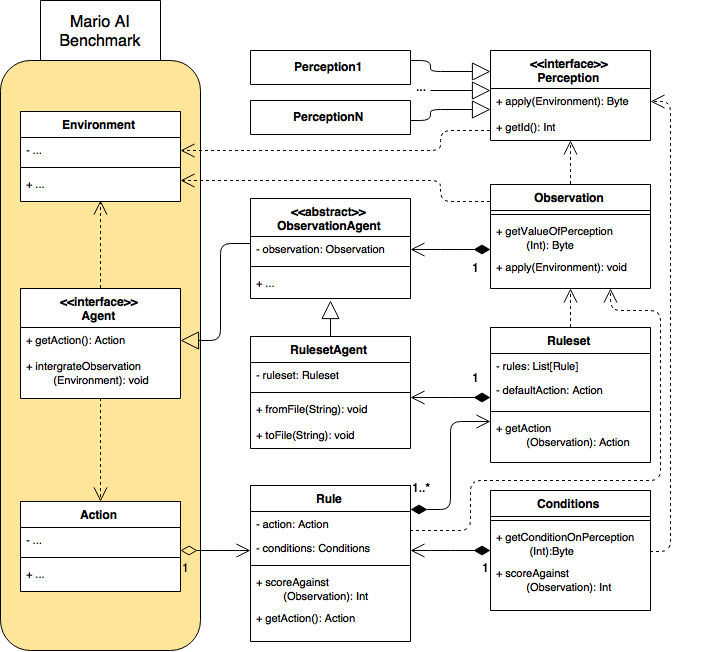
\includegraphics[scale=0.5]{diagrams/AgentClassDiagram.png}
	\caption{UML class diagram of the agent framework.}
	\label{fig:aumlcd}
\end{figure}

The benchmark offers an \emph{Agent} interface, which when extended can be passed into the game playing portion of the software. Every game tick the current \emph{Environment} is passed to the agent, and then the agent is asked for an \emph{Action}, which is a set of explicit key press for Mario to perform.

The agent framework's basis will be extending this interface. Similar to REALM's agent, it will be a rule-based system. A UML class diagram of the system is given in Figure \ref{fig:aumlcd}.

\vspace{\baselineskip}

Each \emph{Agent} instance is initialised with a ruleset, consisting of a list of rules, each containing an \emph{Action}. On receiving the current game \emph{Environment} it is passed to a number of perception objects. Each one is responsible for a exactly one measurement (e.g. Enemy ahead, Mario moving to right etc.). These measurements are collected in to an observation object and stored in the agent.

When asked for an action, the \emph{Agent} passes this observation to its ruleset, which tests it against each rule. Rules contain conditions on what perception measurements should be, which determine its score for a given observation. The highest scoring  rule (with a conflict strategy for ties) is then asked for its action, which is returned from the agent.

\vspace{\baselineskip}

Perceptions are hard coded and as such all of an agents behaviour is determined by its ruleset. If ruleset are implemented in a persistable fashion it ensures that agents can be read and written to external files. Furthermore, rulesets are immutable and only information received during the current game tick is considered. Hence, agents have no state and are deterministic and thread safe (assuming the game engine is).

The capability of this framework is closely tied to the choice of perceptions, which therefore must be chosen with careful consideration. The perceptions chosen were based upon those used in the REALM v1 agent \cite[p.~85]{realm}. The following is the final list of perceptions chosen:
\begin{description}
\item[MarioMode] Measures whether Mario is \textbf{small}, \textbf{big} or \textbf{fire} (capable of throwing fireballs).
\item[JumpAvailable] Detects if Mario has the ability to jump (i.e. on the ground or gripping a wall with the jump key off).
\item[OnGround] Measures whether Mario is in the air or not.
\item[EnemyLeft] Detects if an enemy is to the left of Mario.
\item[EnemyUpperRight] Detects if an enemy is to the upper right of Mario.
\item[EnemyLowerRight] Detects if an enemy is to the lower right or directly to the right of Mario.
\item[ObstacleAhead] Detects if there is a block or terrain directly to the right of Mario.
\item[PitAhead] Detects if there is a pit (falling into pits will end the level) to the right of Mario.
\item[PitBelow] Detects if there is a pit directly below Mario.
\item[MovingX] Measures the direction Mario is moving horizontally.
\item[MovingY] Measures the direction Mario is moving vertically.
\end{description}

The set of actions Mario can take is any combination of 6 key presses: \textbf{left}, \textbf{right}, \textbf{up}, \textbf{down}, \textbf{jump} and \textbf{speed} (which also shoots a fireball if possible). It was decided that this set would be restricted for use in the ruleset agent, only allowing cobinations of \textbf{left}, \textbf{right}, \textbf{jump} and \textbf{speed}. This was to reduce the size of the rules, which reduces the search space of any learning process. The \textbf{up} key performed no function and the \textbf{down} key made Mario crouch, which seemed too niche to be useful during the design process.


%-----------------------------------------------------------------------
% Lang + Tools
%-----------------------------------------------------------------------

\subsection{Language and Tools}

\subsubsection{Scala}
\label{subsec:langchoice}
The dependency on the Mario AI Benchmark restricts the language choice to those that can run on the JVM. Hence, Scala was chosen to be the primary language of the project. It's functional programming elements (pattern matching, list processing etc.) are very applicable to the ruleset and it's semantic reasoner. Scala's focus on immutability aids in maintaining the thread safety requirement. Furthermore, ECJ's structure necessitates the use of type casting, which Scala handles elegantly. Several other Scala features were used throughout the project, such as lambdas, singletons, type aliases and case classes. 

\subsubsection{Maven}
With two major and several minor dependencies, their management is important to the project. Maven was chosen to maintain this, as well as package the main project and both the sub-projects. It was chosen for its ability to package both Java and Scala projects, keeping the tools consistent across the entire code base.


%-----------------------------------------------------------------------
% Impl
%-----------------------------------------------------------------------

\subsection{Implementation}

The design of the agent framework allows for agents to be fully determined by their ruleset. In order for an agent to be used in a evolutionary algorithm it must be represented by a simple data structure. Hence, implementation must allow for agent's rulesets to be unambiguously represented as, for example, a one dimensional collection.

\subsubsection{Perceptions}

The Perception interface was implemented as an abstract class, with an index integer field and an apply method. \emph{apply} takes the game Environment and returns a Byte (8-bit integer) instance, representing the measurement. Perception was extended into two further abstract classes: BoolPerception, which enforces apply's return be either 1 or 0, representing true and false respectively; and BytePerception, which has a limit field and enforces apply's return is between 0 and limit (inclusively).

Concrete perceptions were implemented as objects (singletons) using the \emph{case} keyword, which allows for exhaustive pattern matching on the Perception class, as well as type safe extension by adding further case objects. Each one declares a unique index integer to the Perception superclass (starting at 0 and increasing by one for each). They implement the apply method to return their specific measurement.

For illustration, consider these examples. The perception PitBelow extends BoolPerception, with a unique index of 8 and implements \emph{apply} to return 1 if there is a pit directly below Mario and 0 otherwise. MarioMode extends BytePerception, with a unique index of 0 and a limit of 2, with \emph{apply} returning 0 if Mario is \textbf{small}, 1 for \textbf{big} and 2 for \textbf{fire}.

This approach keeps all the information about perceptions contained in one file. The number of perceptions is easily extended by adding more case objects. Furthermore, it allows the Observation and Conditions classes to be implemented as fixed length byte vectors, with the vector's index matching the perception's unique index field. With use of Scala's implicit and extractor functionality, building the Observation and validating the Conditions vectors is type safe and concise:


\begin{minipage}{0.9\linewidth}
\centering
\begin{lstlisting}
val observationVector = 
    Vector.tabulate(Perception.NUMBER_OF_PERCEPTIONS) {
        n: Int => n match {
            // This retrieves the perception object with the index
            // that matches n. 
            case Perception(perception) => perception(environment)
        }
    }
\end{lstlisting}
\end{minipage}

\begin{minipage}{0.9\linewidth}
\centering
\begin{lstlisting}
def validateConditions(conditionsVector: Vector[Byte]): Boolean = {
    conditionsVector.zipWithIndex.forall {
        case (b: Byte, Perception(perception)) => perception match {
            case boolP : BoolPerception => 
                (b == boolP.TRUE) || (b == boolP.FALSE) 
                    || (b == DONT_CARE)
            case byteP : BytePerception => 
                ((0 <= b) && (b <= byteP.limit)) || (b == DONT_CARE)
        }
        case _ => false 
    }
}

\end{lstlisting}
\end{minipage}

Notice that no information about specific concrete perceptions is required, enforcing the open-closed design principle and allowing perceptions to be added without need to alter this code.

\subsubsection{Perceiving the Environment}

The \emph{Environment} interface contains several individual methods that report Mario's situation. Therefore implementing Perceptions that concerned Mario (e.g. MarioMode, MovingX etc.) was trivial.

Perceptions pertaining to enemies, obstacles or pits was more challenging. Environment provides two 19x19 arrays, one for enemies and one for terrain. Centred around Mario, each array element represents a `square' (16 pixels) of the level scene. The value of an element marks the presence of an enemy or terrain square. 

Enemy and obstacle perceptions pass the relevant array, a lambda test function, coordinates for a box segment of the array and a boolean to a helper function. This function uses Scala's for loop comprehensions to search through the box, applying the lambda to each element, returning the boolean parameter if the lambda returns true at least once. In this way it is easy to search for an enemy or obstacle in a box relative to Mario. Pits work in a similar way, but declare columns instead. If there is no terrain in the column below Mario's height, then it is considered a pit. Take EnemyLeft for example:

\begin{minipage}{0.9\linewidth}
\centering
\begin{lstlisting}
case object EnemyLeft extends BoolPerception(3) {
    // Minus = (Up,Left) | Plus = (Down,Right)
    val AREA_UL = (-2,-2); val AREA_BR = (1, -1);
  
    def apply(environment: Environment): Byte = {
        if(Perception.enemyInBoxRelativeToMario(environment, AREA_UL, AREA_BR)) 
            1 else 0  
    }
}
\end{lstlisting}
\end{minipage}

\begin{minipage}{0.9\linewidth}
\centering
\begin{lstlisting}
def enemyInBoxRelativeToMario(
          environment: Environment, 
          a: (Int, Int), b: (Int, Int)): Boolean = {
    val enemies = environment.getEnemiesObservationZ(2);
    val test = (grid: Array[Array[Byte]], tup: Tuple2[Int, Int]) =>{
         val x = grid(tup._1)(tup._2)
         x == 1
    }
    checkBox(enemies, test, getMarioPos(environment), a, b, true)
}
\end{lstlisting}
\end{minipage}

\begin{minipage}{0.9\linewidth}
\centering
\begin{lstlisting}
def checkBox(grid: Array[Array[Byte]], 
               test: (Array[Array[Byte]], (Int, Int))=>Boolean, 
               mario: (Int, Int), 
               a: (Int, Int), b: (Int, Int), 
               ret: Boolean): Boolean = {
    import Math.min
    import Math.max
    val relARow = min(grid.length-1, max(0, (a._1 + mario._1)))
    val relACol = min(grid(0).length-1, max(0, (a._2 + mario._2)))
    val relBRow = min(grid.length-1, max(0, (b._1 + mario._1)))
    val relBCol = min(grid(0).length-1, max(0, (b._2 + mario._2)))
    
    for {
      i <- min(relARow, relBRow) to max(relARow, relBRow)
      j <- min(relACol, relBCol) to max(relARow, relBCol)
      if (test(grid, (i, j)))
    }{
        return ret
    }
    !ret
}
\end{lstlisting}
\end{minipage}


\subsubsection{Observation, Conditions and Actions}

For clarity an Action class was created for use in the ruleset, with an adapter method to convert it into the boolean array expected in the Agent interface. As the Observation and Conditions classes were to be implemented as fixed length byte vectors, so was the Action class.

Action vectors have a fixed length of 4, where elements represent \textbf{left}, \textbf{right}, \textbf{jump} and \textbf{speed} respectively. Observation vectors have a fixed length equal to the number of perceptions and hold the byte returned by each Perception's apply function. Conditions have the same length and hold data in the same range as Observation, the condition on each perception therefore being that the corresponding element in the observation be equal. They have one additional possible value, {\footnotesize DONT\_CARE} (equal to byte -1), which represents that no condition be placed on that perception.

Instead of implementing these classes as wrappers for \emph{Vector[Byte]}, which can be inefficient and overly verbose, type aliases were used. This allowed each class to be referred to explicitly (rather than just by variable name), which provides readability and type safety, whilst still having direct access to the list processing methods included in the Vector class. They were declared on the agent framework's package object, making them accessible package wide. An object with static data and factory methods was included for each.

For example, this allowed Observation to be used as such:

\begin{minipage}{0.9\linewidth}
\centering
\begin{lstlisting}
abstract class ObservationAgent extends Agent {
    ...
    // Using factory method for a blank observation
    var observation: Observation = Observation.BLANK
    ...
    def integrateObservation{env: Environment}: Unit = {
        // Using the Observation factory method 
        // to build a new observation
        observation = Observation(env)
        
        if (printObservation) {
            // Using Vector method foreach directly
            observation.foreach { 
                b:Byte => print(" ~ " + b)
            }
        } 
        ...
    }
    ...
 }

\end{lstlisting}
\end{minipage}


\subsubsection{Rules and Rulesets}

Having both Conditions and Action implemented as byte vectors allows rules to be represented in the same way. Each rule is simple the concatenation of the Conditions and Action vectors. The rule vector are fixed length as both Conditions and Action are. Moreover, as rulesets contain just a list of rules, rulesets can be unambiguously represented by a single dimension byte vector. This allows rulesets not only to be persisted easily (as say a csv) but also gives the data representation needed for the evolutionary process.

In this case both Rule and Ruleset were implemented as wrapper classes for \emph{Vector[Byte]} and \emph{Seq[Rule]} respectively. Ruleset also holds a default Action, which is used if no rule matches the environment.

The semantic reasoner of the rule system is split across both classes. In Rule, the \emph{scoreAgainst} method is passed the observation and produces a score by looping through the conditions and adding 1 if the condition and observation match in value and 0 if the condition is {\footnotesize DONT\_CARE}. If a mismatched condition is found, the method immediately returns with -1. It is implemented tail recursively to provide maximum efficiency.

\begin{minipage}{0.9\linewidth}
\centering
\begin{lstlisting}
def scoreAgainst(observation: Observation): Int = {
    val conditions = ruleVector.slice(0, Conditions.LENGTH)
    @tailrec
    def scoreRecu(i: Int, sum: Int = 0): Int =  {
        if (i == Conditions.LENGTH) sum
        else conditions(i) match {
            case Conditions.DONT_CARE => scoreRecu(i+1, sum)
            case b if b == observation(i) => scoreRecu(i+1, sum+1)
            case _ => -1
        }
    }
    scoreRecu(0)
}
\end{lstlisting}
\end{minipage}

In Ruleset, the \emph{getBestAction} is passed the observation and returns an action boolean array. Using tail recursion it performs a fold operation on its rules, saving and returning the best scoring rule (preferring earlier rules when tied). If no rule gets a score of 0 or above then the default action is returned.

\begin{minipage}{0.9\linewidth}
\centering
\begin{lstlisting}
def getBestExAction(observation: Observation): Array[Boolean] = {
    
    @tailrec
    def getBestRuleRecu(rs: Seq[Rule], best: Option[Rule] = None, bestScore: Int = 0): Option[Rule] = 
        rs match {
          case Nil => best
          case (r +: ts) => {
              val newScore = r.scoreAgainst(observation)
              if (newRuleBetter(bestScore, newScore))
                  getBestRuleRecu(ts, Some(r), newScore)
              else
                  getBestRuleRecu(ts, best, bestScore)
        }
    }
    
    getBestRuleRecu(rules) match {
        case None => defaultAction.toBooleanArray
        case Some(r) => r.getAction.toBooleanArray
    }
}
\end{lstlisting}
\end{minipage}


\subsubsection{Persistence}

Agent's are persisted by persisting their ruleset. Rulesets are persisted in single line csv files. An IO helper object is passed an agent, extracts it's ruleset and requests it's vector representation, writing each byte separated by a comma. On reading an agent file, it constructs a byte vector. This byte vector is passed to the Ruleset's factory method, which groups the vector by rule length to form the rule sequence.

%-----------------------------------------------------------------------
% Testing
%-----------------------------------------------------------------------

\subsection{Testing}

Due to the agent modules heavy reliance of the Environment interface the use of a mocking facility was required. The ScalaMock testing library was adding to the project to provide this.

Perceptions were unit tested individually, using white-box approach (due to the inclusion of mocking). Each test stubbed the Environment interface, instructing it to return a specific value (or array) for the relevant call, and testing that the perception echoed or processed it correctly. This allowed Perceptions to be tested independently of the game engine and provided test coverage. However, as there was very little documentation Environment interface, expected return values had to be investigated manually and edge cases could have easily been missed.

Rulesets (and Rules) were tested with a largely black-box end-to-end style. This was required due to the reliance of type aliases. Fixed rulesets were constructed to verify that the \emph{getAction} method returned the expected action based on a fixed observation. Mocking of individual rules was not used in case the Rule class was altered to be a type alias instead of a wrapper class.

These tests were added to Maven's build lifecycle, and hence run on every project build.

%-----------------------------------------------------------------------
% Handcrafted
%-----------------------------------------------------------------------

\subsection{Handcrafted Agents}

For the purpose of evaluation and comparison three handcrafted rulesets were created for the agent framework.

\begin{description}
	\item[Forward Jumping] This ruleset commands the agent to jump whenever it can, regardless of its surroundings. It contains a single rule and a default action. It is a blind agent that does not take advantage of the framework, however it is surprising effective. An analogous agent was used for comparisons in the 2009 Mario AI Competition and was found to score higher than many entrants. The learning process will aim to discourage this behaviour as it is neither interesting or optimal.
	\item[Simple Reactive] This agent only jumps when it detects an enemy, obstacle or pit in its way. It contains 5 rules and defaults to moving right at speed. This agent makes better use of the framework, but still does not use all of its perceptions. Its behaviour is more interesting, however it tends to score similarly to the forward jumping agent. Despite low attainment, a learnt agent that behaves in a similar way will be evaluating more favourably as it is using more of the agent's perceptions.
	\item[Complex] This agent is the most interesting and highest scoring of the three. It has several different behaviours and builds off of the simple reactive agent. It contains 18 rules and makes use of all perceptions except MarioMode and EnemyLeft. Its behaviour was investigated at length and as such will form a good comparison to the final learnt agent. Effective evolved behaviours unconsidered in this agent's creation are a sign of the validity of the learning process. 
\end{description}
Creation of the handcrafted rulesets also informed additions and alterations to the agent's perceptions. For example, it was originally difficult to create an effective pit strategy and so PitAhead was changed from a BoolPerception to a BytePerception, returning 3 values representing \textbf{none}, \textbf{far} and \textbf{close}.
!PUT RULESETS IN APPENDIX?!


%___________________________________________
%*************************************************************
% Level Playing
%___________________________________________
%^^^^^^^^^^^^^^^^^^^^^^^^^^^^^^^^^^^^^^^^^^^^^^^^^^^

\section{Level Playing Module}

The main purpose of the level playing module is to evaluate the fitness of agents during the learning process. An effective learning process needs a diverse testbed, thus the level playing module must be deterministic, highly configurable and able to provide variety. 

%-----------------------------------------------------------------------
% Design
%-----------------------------------------------------------------------

\subsection{Design}

\begin{figure}[t]
	\centering
	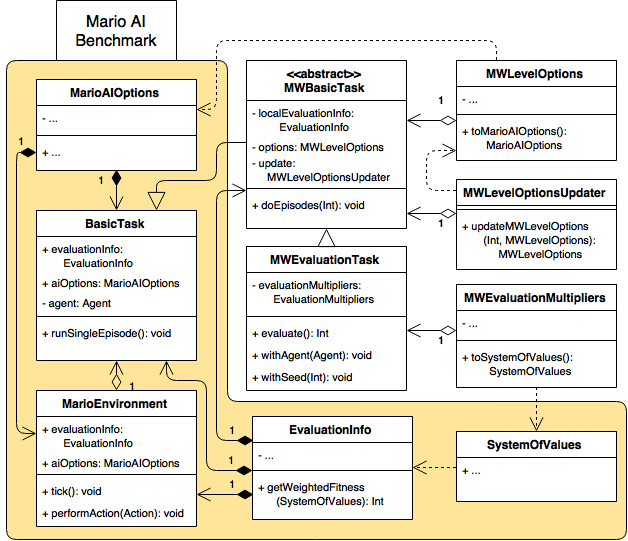
\includegraphics[scale=0.5]{diagrams/PlayingClassDiagram.png}
	\caption{UML class diagram of the level playing module.}
	\label{fig:pumlcd}
\end{figure}

In the benchmark the heart of the game engine is the \emph{MarioEnvironment} class. It is responsible for calling the \emph{LevelGeneration} class, updating the scene each tick with an action, and reporting the scene through the Environment interface. Parameters controlling level generation and playing are contained in the \emph{MarioAIOptions} class. The \emph{BasicTask} class controls the game loop in conjunction with an agent. It initialises the MarioEnvironment class with options, then runs through the loop, commanding a tick, passing the environment to the agent and finally requesting an action and passing it to the MarioEnvironment instance. Statistics pertaining to the agents performance are stored in MarioEnvironment in the \emph{EvaluationInfo} class, which are cloned to BasicTask at the end of the level. Fitness can be requested from EvaluationInfo with the optional parameter, a \emph{SystemOfValues} instance, which contains the multipliers for various measurements.

The MarioAIOptions class contains several useful parameters. They include: a integer seed, which is passed to the level generator's RNGs; a boolean that toggles visualisation; integers that determine level difficulty, length and time-limit; and booleans that toggle enemies, pits and blocks. The SystemOfValues class contains multipliers for  distance achieved, whether or not the level was completed, the amount of time left on completion as well as many others.

\vspace{\baselineskip}

The level playing module will extend this system. It's primary objective will be to allow for multiple levels (episodes) to be played with options that update as prescribed by some parameter class. Upon completion it will produce a fitness based on all levels played. Furthermore, it will allow for the injection of different agents and level seeds, to allow different agents to play the same options without rebuilding the instance. A UML class diagram for the module can be found in Figure \ref{fig:pumlcd}.

Level options are stored in the \emph{MWLevelOptions} class, which acts as an adapter for the MarioAIOptions class. Each new level these will be updated by the dedicated \emph{MWLevelOptionsUpdater} class. The \emph{EvaluationMultipliers} class is an adapter for the SystemOfValues class, which is used to calculate the fitness at the end of a sequence of levels. Both MWLevelOptions and EvaluationMultipliers are designed to be data classes, which provides determinism and thread safety, as well as easy persistence. MWLevelOptionsUpdater's qualities in this regard are Implementation details and are discussed in a following section. The full list of parameters held in these classes can be found in the Appendix !REF!.


%-----------------------------------------------------------------------
% Implementation
%-----------------------------------------------------------------------

\subsection{Implementation}

\subsubsection{Parameter Classes}

The MWLevelOptions and MWEvaluationMultipliers classes were implemented as data classes in an immutable builder pattern style. Each field has a \emph{withField(field)} method that returns a cloned instance with that field changed. This affords a concise, declarative style, whilst maintaining immutability. MWEvaluationMultipliers has a implicit converter to a SystemOfValues instance, which is required for evaluation in the benchmark. However, a similar approach was not possible for converting MWLevelOptions to a MarioAIOptions instance (required for the game-engine). MarioAIOptions hold more parameters than MWLevelOptions (e.g. agent and level seed), therefore the adapter function takes both the current MarioAIOptions and a MWLevelOptions instance as parameters and updates the former by overriding the corresponding fields with values from the latter.

MWLevelOptions was not implemented as a class. Instead, MWBasicTask expects a lambda function. This lambda takes the episode number and the current MWLevelOptions, returning an updated set of options. MWLevelOptions builder structure ensures this is always a new instance, and hence maintains immutability. The inclusion of the episode number allows the function to remain deterministic. Moreover, with the ability to build closures in Scala, this lambda can be built from data (for example, a list of options, where indexes relate to episode number).

\subsubsection{Persistence}

The primary use of the level playing module is during the evaluation stage of the learning process. Hence, it was decided to use ECJ's parameter file system to persist level playing parameters, which allows them to be written in the same file as the rest of the learning parameters.

ECJ's parameter system builds upon Java's Properties file system. From a parameter file (formatted in the Java Properties format) a ParameterDatabase can be built, from which specific parameters can be requested using the Parameter class. This system was used to persist the two parameter classes, MWLevelOptions and MWEvaluationMultipliers; the level options update lambda data; and other level playing data such as number of levels (episodes) and base level seed. For example, the following lines would set the number of levels to 10 and the base difficulty to 5:

\begin{minipage}{0.9\linewidth}
\centering
\begin{lstlisting}
          level.num-levels = 10
level.base.difficulty-num = 5
\end{lstlisting}
\end{minipage}

A static utility class EvaluationParamsUtil was created to handle the reading of the level playing data from these files. A ParameterDatabase is built and passed to utility class, which builds the required parameter class. For MWLevelOptions and MWEvaluationMultipliers it searches for the prefixes `{\ttfamily level.base}' and `{\ttfamily mult}' respectively and then looks for suffixes corresponding to specific fields. If a field's suffix is not found then it is initialised to a default value (which is always zero for MWEvaluationMutlipliers).

The update lambda is built as a closure on a collection of Map instances, one for each field in MWLevelOptions. For each {\ttfamily n} from 0 to the number of levels (episodes), the utility function looks for the prefix `{\ttfamily level.{n}}', which is used to hold the update for episode \textbf{n}. For each field a Map is built and using the same suffixes as for MWLevelOptions, key-value pairs are added mapping \textbf{n} to the value found. When the update lambda is called, it consults these maps and updates the MWLevelOptions with the new value if one is found for the current episode number.

For example, if the parameter file contained the following lines:

\begin{minipage}{0.9\linewidth}
\centering
\begin{lstlisting}
   level.num-levels = 4
 level.base.enemies = false
    level.1.enemies = true
    level.3.enemies = false
\end{lstlisting}
\end{minipage}

Then enemies would be off for the first episode, on for the second and third and off again for the fourth and final episode.

\subsubsection{The Episode Loop}

The entry point of the level playing module is the MWEvaluationTask class, which extends the abstract MWBasicTask class. MWEvaluationTask is instantiates with a base set of options (as MWLevelOptions), a MWEvaluationMutlipliers instance and an update lambda, as well as the number of episodes (levels) to run. The agent and base level seed can be injected with the \emph{withAgent(agent)} and \emph{withLevelSeed(seed)} methods (which also reset of evaluation information).

\begin{minipage}{0.9\linewidth}
\centering
\begin{lstlisting}

class MWEvaluationTask(val numberOfLevels: Int, 
                       val evalValues: MWEvaluationMultipliers, 
                       override val baseLevelOptions: MWLevelOptions, 
                       override val updateOptionsFunc: (Int, MWLevelOptions) => MWLevelOptions)
                           extends MWBasicTask("MWMainPlayTask", baseLevelOptions, updateOptionsFunc, visualisation, args) with EvaluationTask {

    private var baseLevelSeed: Int = 0;
    
    override def nextLevelSeed(episode: Int, lastSeed: Int) =  {
        (3*episode) + lastSeed
    }    
        
    override def evaluate: Int = {
        doEpisodes
        localEvaluationInfo.computeWeightedFitness(evalValues)
    }
  
    override def withAgent(agent: Agent): MWEvaluationTask = {
        super.injectAgent(agent, true)
        this
    }
    
    override def withLevelSeed(seed: Int): MWEvaluationTask = {
        baseLevelSeed = seed
        super.injectLevelSeed(seed, true)
        this
    }
}
\end{lstlisting}
\end{minipage}  

On calling the \emph{evaluate()} method, the number of levels is passed to the \emph{doEpisodes(numberOfEpisode)} (a superclass method), which loops as follows:

\begin{minipage}{0.9\linewidth}
\centering
\begin{lstlisting}

def doEpisodes(amount: Int): Unit = {
    @tailrec
    def runSingle(iteration: Int, prevOptions: MWLevelOptions, disqualifications: Int): Int = {
        if (iteration == amount) { 
            disqualifications
        } else {
            // Calls the update lambda to get episodes set of options
            val newOptions = updateOptions(iteration, prevOptions)
            
            // Converts options to class required for game-engine
            val marioAIOptions = MWLevelOptions.updateMarioAIOptions(super.options, newOptions)
            
            // Updates the level seed (which is set to increase each episode by MWEvaluationClass)
            // Agent instance is already being held here
            marioAIOptions.setLevelRandSeed(nextLevelSeed(iteration, marioAIOptions.getLevelRandSeed))
            
            // Resets the evaluation information in the super class
            super.setOptionsAndReset(marioAIOptions)

            // Generates and runs the level using the super class
            // Returns true if the agent was not disqualified (took too long to return an action)
            val notDisqualified: Boolean = runSingleEpisode(1)
            val disqualification: Int = if (!notDisqualified) 1 else 0
       
            // Update the evaluation information for the entire run
            // (as the super classes evaluationInfo gets reset every level
            updateLocalEvaluationInfo(super.getEvaluationInfo)
            
            // Loop
            runSingle(iteration+1, newOptions, disqualifications + disqualified)
        }
    }
    
    // Sets the base options
    super.setOptionsAndReset(MWLevelOptions.updateMarioAIOptions(options, baseLevelOptions))
    disqualifications = runSingle(0, baseLevelOptions, 0)
}
\end{lstlisting}
\end{minipage}


Before every episode the options are updated by the lambda, updating the base options in the first episode. A new level seed is also requested from the MWEvaluationClass, which simply increases it each episode. These updates are converted and added to a MarioAIOptions instance and passed to the superclass in the benchmark. A single level is then generated and played using the superclass. Evaluation information is added to MWBasicTask's local evaluation information (as the former is reset every episode) and the function loops tail recursively.

When the number of loops equals the number of levels the function exits. At this point the \emph{evaluate()} method requests a fitness from the local evaluation information, passing in the evaluation multipliers, which is then returned.

%-----------------------------------------------------------------------
% Benchmark Edit
%-----------------------------------------------------------------------

\subsection{Modifying the Benchmark}

Preliminary runs of the benchmark software revealed several issues and defects. As the learning algorithm would run over several generations, any errors could halt it prematurely, which could be costly in terms of project time keeping. In order to address this a Java project was created from the benchmark's source code and fixes were made. This code was packaged with Maven and included as a dependency in the main project.

Several minor exceptions were caught or addressed, however the two largest issues failed `quietly'. They concerned the LevelGeneration class and surrounded enemy and pit generation in regards to level difficulty. Fixes were made to ensure level difficulty scaled more consistently.

\subsubsection{Enemy Generation}

In observing the benchmark generated levels it was apparent that enemy density was very high, even on lowest difficulties. Examining the LevelGeneration class revealed this to the result of what was probably unintended behaviour. 

Levels are generated in zones of varying length. Quite often, a zero length zone is created, which has no effect on terrain. However, enemies were still being added to these zones, creating very high density columns of enemies during levels. This was addressed, with the addition of a more gentle enemy count curve and better spacing.

\subsubsection{Pit Generation}

Another apparent shortcoming was pit length. Pits were only of two sizes, small and very large, and after a certain level difficulty were always very large. Although this was intended behaviour, comments from the original developers suggest it was a placeholder for a more sophisticated system. An edit was made to scale maximum pit length on level difficulty. Each pit's length is chosen probabilistically on a bell curve, which is shifted by level difficulty.


%-----------------------------------------------------------------------
% Testing
%-----------------------------------------------------------------------

\subsection{Testing}

!IN PROGRESS!

\subsection{Comparator Task}


%___________________________________________
%*************************************************************
% Learning
%___________________________________________
%^^^^^^^^^^^^^^^^^^^^^^^^^^^^^^^^^^^^^^^^^^^^^^^^^^^

\section{Learning}


%-----------------------------------------------------------------------
% Design
%-----------------------------------------------------------------------

\subsection{Design}


%-----------------------------------------------------------------------
% Modifying the ECJ Library
%-----------------------------------------------------------------------

\subsection{Modifying the ECJ Library}


%-----------------------------------------------------------------------
% Implementation
%-----------------------------------------------------------------------

\subsection{Implementation}


%-----------------------------------------------------------------------
% Testing
%-----------------------------------------------------------------------

\subsection{Testing}


%-----------------------------------------------------------------------
% Parameters
%-----------------------------------------------------------------------

\subsection{Parameters}


%___________________________________________
%*************************************************************
% Evaluation
%___________________________________________
%^^^^^^^^^^^^^^^^^^^^^^^^^^^^^^^^^^^^^^^^^^^^^^^^^^^

\section{Evaluation}


%-----------------------------------------------------------------------
% Agent Framework}
%-----------------------------------------------------------------------

\subsection{Agent Framework}


%-----------------------------------------------------------------------
% Learning
%-----------------------------------------------------------------------

\subsection{Learning}


%-----------------------------------------------------------------------
% Project Evaluation
%-----------------------------------------------------------------------

\subsection{Project Evaluation}

\clearpage
\begin{thebibliography}{11}

\bibitem{myangelcafe}
  Siyuan Xu,
  \emph{History of AI design in video games and its development in RTS games},
  Department of Interactive Media \& Game development, Worcester Polytechnic Institute, USA,
  \url{https://sites.google.com/site/myangelcafe/articles/history_ai}.

\bibitem{pacmanghosts}
  Chad Birch,
  \emph{Understanding Pac-Man Ghost Behaviour},
  \url{http://gameinternals.com/post/2072558330/understanding-pac-man-ghost-behavior},
  2010.
  
\bibitem{halflife}
  Alex J. Champandard,
  \emph{The AI From Half-Like's SDK in Retrospective},
  \url{http://aigamedev.com/open/article/halflife-sdk/},
  2008.
  
\bibitem{fear}
  Tommy Thompson,
  \emph{Facing Your Fear},
  \url{http://t2thompson.com/2014/03/02/facing-your-fear/},
  2014.

\bibitem{halo}
  Damian Isla,
  \emph{GDC 2005 Proceeding: Handling Complexity in the Halo 2 AI},
  \url{http://www.gamasutra.com/view/feature/130663/gdc_2005_proceeding_handling_.php},
  2005.
  
\bibitem{rome}
  Alex J. Champandard,
 \emph{Monte-Carlo Tree Search in TOTAL WAR: Rome II Campaign AI},
 \url{http://aigamedev.com/open/coverage/mcts-rome-ii/},
 2014.
 
\bibitem{playermod}
  Georgios N. Yannakakis, Pieter Spronck, Daniele Loiacono and Elisabeth Andre,
  \emph{Player Modelling},
  \url{http://yannakakis.net/wp-content/uploads/2013/08/pm_submitted_final.pdf},
  2013.
  
\bibitem{skyrim}
  Matt Bertz,
  \emph{The Technology Behind The Elder Scrolls V: Skyrim},
  \url{http://www.gameinformer.com/games/the_elder_scrolls_v_skyrim/b/xbox360/archive/2011/01/17/the-technology-behind-elder-scrolls-v-skyrim.aspx},
  2011.
  
\bibitem{overmind}
  \emph{The Berkeley Overmind Project},
  University of Berkeley, California.
  \url{http://overmind.cs.berkeley.edu/}.
  
\bibitem{cellz}
  Simon M. Lucas,
  \emph{Cellz: A simple dynamical game for testing evolutionary algorithms},
  Department of Computer Science, University of Essex, Colchester, Essex, UK,
  \url{http://citeseerx.ist.psu.edu/viewdoc/download?doi=10.1.1.96.5068&rep=rep1&type=pdf}. 
  
\bibitem{panorama}
  G. N. Yannakakis and J. Togelius,
  \emph{A Panorama of Artificial and Computational Intelligence in Games},
  IEEE Transactions on Computational Intelligence and AI in Games,
  \url{http://yannakakis.net/wp-content/uploads/2014/07/panorama_submitted.pdf},
  2014.
  
\bibitem{marioaicomp}
  Julian Togelius, Noor Shaker, Sergey Karakovskiy and Georgios N. Yannakakis,
  \emph{The Mario AI Championship 2009-2012},
  AI Magazine 34 (3), pp. 89-92,
  \url{http://noorshaker.com/docs/theMarioAI.pdf},
  2013.

\bibitem{suttonrl}
  Richard S. Sutton and Andrew G. Barto,
  \emph{Reinforcement Learning: An Introduction}
  The MIT Press, Cambridge, Massachusetts, London, England,
  Available: \url{http://webdocs.cs.ualberta.ca/~sutton/book/ebook/the-book.html},
  1998.

\bibitem{ev-comp} 
  Gary B. Fogel et al.,
  \emph{Evolutionary Programming}
  Scholarpedia, 6(4):1818.,
  \url{http://www.scholarpedia.org/article/Evolutionary_programming},
  2011.
  
\bibitem{modernai3}
  Stuart J. Russell, Peter Norvig,
  \emph{Artificial Intelligence: A Moden Approach (3rd ed.},
  Upper Saddle River, New Jersey,
  2009.
  
\bibitem{modernai1}
  Stuart J. Russell, Peter Norvig,
  \emph{Artificial Intelligence: A Moden Approach (1st ed.},
  Upper Saddle River, New Jersey,
  1995.
  
\bibitem{rbsys}
  Anoop Gupta, Charles Forgy, Allen Newell, and Robert Wedig,
  \emph{Parallel Algorithms and Architectures for Rule-Based Systems},
  Carnegie-Mellon University Pittsburgh, Pennsylvania,
  ISCA '86 Proceedings of the 13th annual international symposium on Computer architecture, pp.~28-37,
  1986.
  
\bibitem{mitchellga}
  Melanie Mitchell,
  \emph{An Introduction to Genetic Algorithms},
  Cambridge, MA: MIT Press,
  1996.

\bibitem{es-book}
  Hans-Georg Beyer and Hans-Paul Schwefel,
  \emph{Evolution Strategies: A Comprehensive Introduction},
  Natural Computing 1: 3?52,
  2002.

\bibitem{rlheli}
  Andrew Y. Ng, Adam Coates, Mark Diel, Varun Ganapathi, Jamie Schulte, Ben Tse, Eric Berger and Eric Liang,
  \emph{Inverted autonomous helicopter flight via reinforcement learning},
  International Symposium on Experimental Robotics,
  \url{http://www.robotics.stanford.edu/~ang/papers/iser04-invertedflight.pdf},
  2004.
  
\bibitem{rlhci}
  S. Singh, D. Litman, M. Kearns and M. Walker,
  \emph{Optimizing Dialogue Management with Reinforcement Learning: Experiments with the NJFun System},
  Journal of Artificial Intelligence Research (JAIR), Volume 16, pages 105-133, 2002,
  \url{http://web.eecs.umich.edu/~baveja/Papers/RLDSjair.pdf}.
  
\bibitem{evolutioningamedesign}
  Alex J. Champandard,
  \emph{Making Designers Obsolete? Evolution in Game Design},
  \url{http://aigamedev.com/open/interview/evolution-in-cityconquest/},
  2012.
  
\bibitem{blackandwhite}
  James Wexler,
  \emph{A look at the smarts behind Lionhead Studio's `Black and White' and where it can and will go in the future},
  University of Rochester, Rochester, NY 14627,
  \url{http://www.cs.rochester.edu/~brown/242/assts/termprojs/games.pdf},
  2002.
  
\bibitem{projectgothamracing}
  Thore Graepal (Ralf Herbrich, Mykel Kockenderfer, David Stern, Phil Trelford),
  \emph{Learning to Play: Machine Learning in Games},
  Applied Games Group, Microsoft Research Cambridge,
  \url{http://www.admin.cam.ac.uk/offices/research/documents/local/events/downloads/tm/06_ThoreGraepel.pdf}.
  
\bibitem{forza}
  \emph{Drivatar\texttrademark\ in Forza Motorsport},
  \url{http://research.microsoft.com/en-us/projects/drivatar/forza.aspx}.
  
\bibitem{2012the}
  Sergey Karakovskiy and Julian Togelius,
  \emph{Mario AI Benchmark and Competitions},
  \url{http://julian.togelius.com/Karakovskiy2012The.pdf},
  2012.
  
\bibitem{2010the}
  Julian Togelius, Sergey Karakovskiy and Robin Baumgarten,
  \emph{The 2009 Mario AI Competition},
  \url{http://julian.togelius.com/Togelius2010The.pdf},
  2010.
  
\bibitem{2014how}
  Julian Togelius,
  \emph{How to run a successful game-based AI competition},
  \url{http://julian.togelius.com/Togelius2014How.pdf},
  2014.
  
\bibitem{torcs}
  \emph{TORCS: The Open Racing Car Simulation},
  \url{http://torcs.sourceforge.net/}.

\bibitem{scrc}
  Daniele Loiacono, Pier Luca Lanzi, Julian Togelius, Enrique Onieva, David A. Pelta, Martin V. Butz, Thies D. L�nneker, Luigi Cardamone, Diego Perez, Yago S�ez, Mike Preuss, and Jan Quadflieg,
  \emph{The 2009 Simulated Car Racing Championship},
  IEEE Transactions on Computational Intelligence and AI in Games, VOL. 2, NO. 2,
  2010.
  
\bibitem{2kbot}
  \emph{The 2K BotPrize},
  \url{http://botprize.org/}
  
\bibitem{starcomp}
  Michael Buro, David Churchill,
  \emph{Real-Time Strategy Game Competitions},
  Association for the Advancement of Artificial Intelligence, AI Magazine, pp.~106-108,
  \url{https://skatgame.net/mburo/ps/aaai-competition-report-2012.pdf},
  2012.
  
\bibitem{imb}
  \emph{Infinite Mario Bros.},
  Created by Markus Perrson,
  \url{http://www.pcmariogames.com/infinite-mario.php}.
  
\bibitem{handa}
  H. Handa,
  \emph{Dimensionality reduction of scene and enemy information in mario},
  Proceedings of the IEEE Congress on Evolutionary Computation,  
  2011.
  
\bibitem{rossbagnell}
  S. Ross and J. A. Bagnell, 
  \emph{Efficient reductions for imitation learning},
  International Conference on Artificial Intelligence and Statistics (AISTATS),
  2010.
  
\bibitem{realm}
  Slawomir Bojarski and Clare Bates Congdon,
  \emph{REALM: A Rule-Based Evolutionary Computation Agent that Learns to Play Mario},
  2010 IEEE Conference on Computational Intelligence and Games (CIG '10) pp.~83-90.

\bibitem{gramev}
   D. Perez, M. Nicolau, M. O'Neill, and A. Brabazon,
   \emph{Evolving Behaviour Trees for the Mario AI Competition Using Grammatical Evolution},
   Proceedings of EvoApps, 2010, pp.~123-132.

\bibitem{feetsies}
  E. R. Speed, 
  \emph{Evolving a mario agent using cuckoo search and softmax heuristics},
  Proceedings of the IEEE Consumer Electronics Society's Games Innovations Conference (ICE-GIC), 2010,
  pp.~1-7.
  
\bibitem{emapf}
  Thomas Willer Sandberg,
  \emph{Evolutionary Multi-Agent Potential Field based AI approach for SSC scenarios in RTS games},
   University of Copenhagen,
   2011.
  
\bibitem{ecj}
  \emph{ECJ: A Java-based Evolutionary Computation Research System},
  \url{https://cs.gmu.edu/~eclab/projects/ecj/}.
  
\bibitem{ecj-manual}
  Sean Luke,
  \emph{The ECJ Owner's Manual, v23},
  \url{https://cs.gmu.edu/~eclab/projects/ecj/docs/manual/manual.pdf}
  George Mason University,
  2015.
  
\bibitem{jgap}
  \emph{JGAP: Java Genetic Algorithms Package},
  \url{http://jgap.sourceforge.net/}.

\bibitem{astar}
  Robin Baumgarten,
  \emph{A* Mario Agent},
  \url{https://github.com/jumoel/mario-astar-robinbaumgarten}.
  
\bibitem{agentsmith}
  Ryan Small,
  \emph{Agent Smith: a Real-Time Game-Playing Agent for Interactive Dynamic Games},
  GECCO `08, July 12-16, 2008, Atlanta, Georgia, USA.
  \url{http://www.cs.bham.ac.uk/~wbl/biblio/gecco2008/docs/p1839.pdf}.

\end{thebibliography}
\end{document}

























